\section{Results}
\label{sec:results}

\subsection{Primary Finding: Alignment Signal Fails on Both Datasets}

Table~\ref{tab:main} reports gradient alignment vs.\ per-sample loss ROC-AUC at checkpoint epochs.

\begin{table}[h]
\centering
\caption{Gradient alignment vs.\ per-sample loss ROC-AUC at checkpoint epochs. $\dagger$ Gap = Align $-$ Loss; negative values indicate alignment below loss (expected direction of failure).}
\label{tab:main}
\begin{tabular}{lcccccc}
\toprule
\textbf{Epoch} & \textbf{WB Align} & \textbf{WB Loss} & \textbf{WB Gap}$^\dagger$ & \textbf{CelebA Align} & \textbf{CelebA Loss} & \textbf{CelebA Gap}$^\dagger$ \\
\midrule
1  & 0.150 & 0.930 & $-$0.780 & 0.246 & 0.975 & $-$0.729 \\
5  & 0.301 & 0.854 & $-$0.554 & 0.484 & 0.949 & $-$0.465 \\
10 & 0.340 & 0.821 & $-$0.481 & 0.523 & 0.939 & $-$0.416 \\
25 & 0.340 & 0.801 & $-$0.461 & 0.407 & 0.910 & $-$0.503 \\
50 & 0.349 & 0.775 & $-$0.426 & 0.632 & 0.905 & $-$0.273 \\
\bottomrule
\end{tabular}
\end{table}

\begin{figure}[h]
\centering
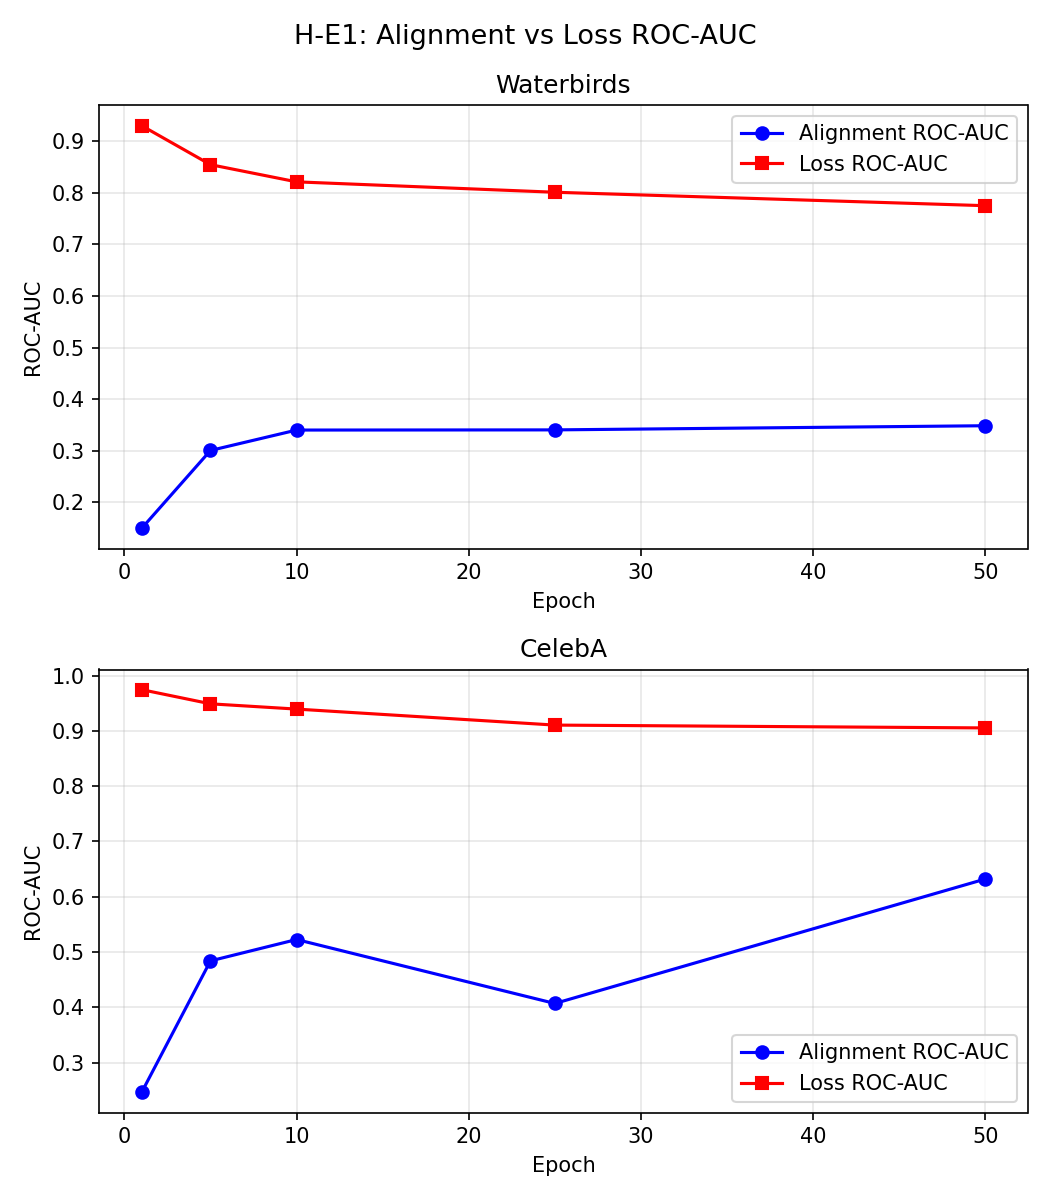
\includegraphics[width=0.85\linewidth]{figures/roc_auc_vs_epoch.png}
\caption{ROC-AUC vs.\ training epoch for gradient alignment score and per-sample loss, on Waterbirds (solid lines) and CelebA (dashed lines). Alignment ROC-AUC (blue) remains far below loss ROC-AUC (orange) at all epochs. Dotted horizontal line at 0.5 marks chance; alignment falls below chance on Waterbirds throughout training.}
\label{fig:roc_epoch_combined}
\end{figure}

\begin{figure}[h]
\centering
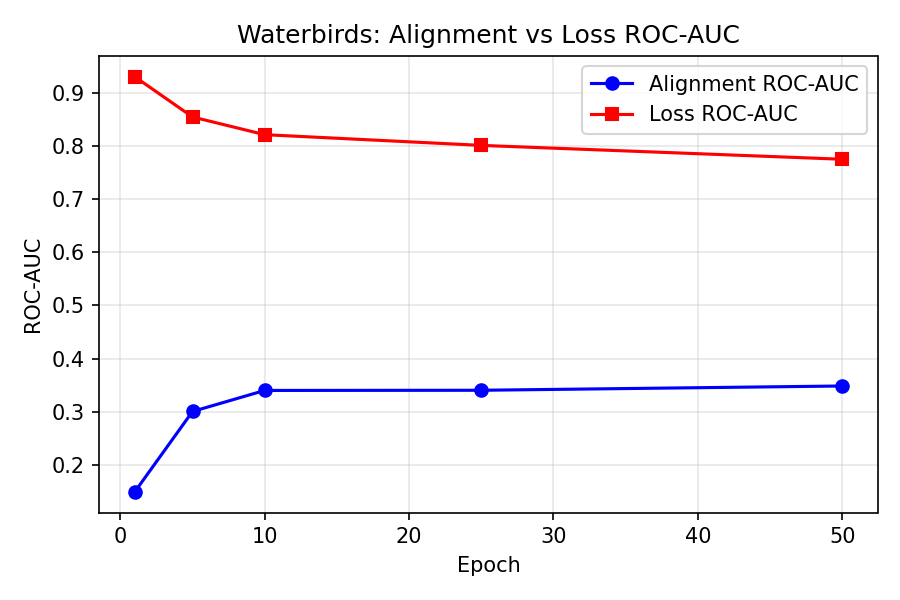
\includegraphics[width=0.85\linewidth]{figures/roc_auc_vs_epoch_waterbirds.png}
\caption{Waterbirds detail. Alignment ROC-AUC (0.150--0.349) vs.\ loss ROC-AUC (0.775--0.930) across epochs 1--50. Alignment begins below chance (0.5) and never approaches it.}
\label{fig:roc_epoch_wb}
\end{figure}

\begin{figure}[h]
\centering
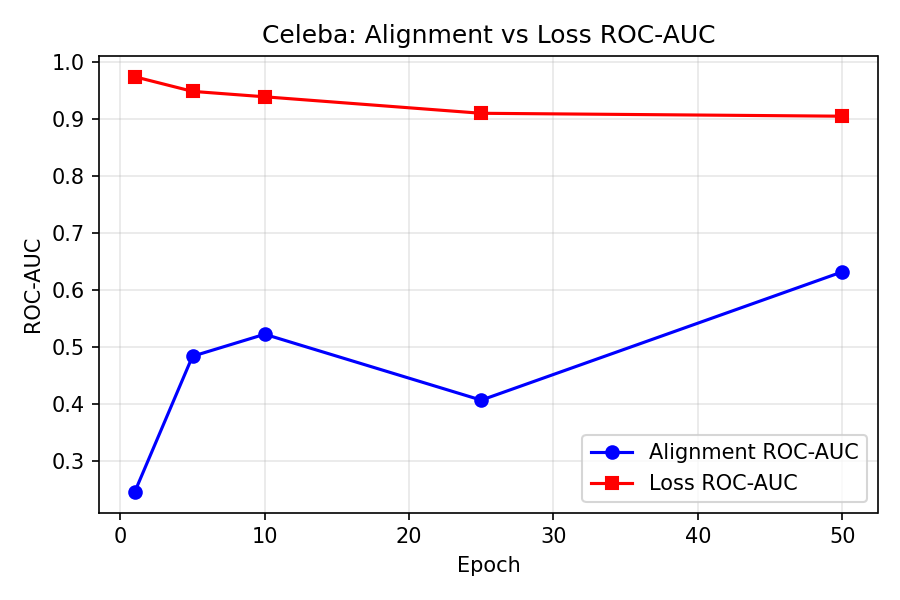
\includegraphics[width=0.85\linewidth]{figures/roc_auc_vs_epoch_celeba.png}
\caption{CelebA detail. Alignment ROC-AUC (0.246--0.632) vs.\ loss ROC-AUC (0.905--0.975) across epochs 1--50. Alignment shows a non-monotonic trajectory, dipping at epoch~25 before recovering. Gap at best alignment epoch~(50): 0.273.}
\label{fig:roc_epoch_celeba}
\end{figure}

\subsection{The Alignment Inversion Effect on Waterbirds}

At epoch~1 on Waterbirds: alignment ROC-AUC = \textbf{0.150}, substantially below chance (0.5).
The conflict score $a_i$ (negated cosine similarity) is anti-predictive: minority samples score \emph{lower} on $a_i$ than majority samples, meaning minority samples have \emph{higher} raw cosine similarity with the within-batch mean --- the direct opposite of the hypothesis.
The inversion partially recovers by epoch~50 (0.349) but alignment never exceeds 0.35 at any tested epoch.
The gap to loss remains 0.43--0.78 throughout training.

\subsection{Temporal Dynamics}

On Waterbirds, per-sample loss ROC-AUC begins high (0.930 at epoch~1) and monotonically degrades to 0.775 at epoch~50 as the model memorizes training samples.
Gradient alignment begins inverted and slowly improves --- converging toward loss from below, as training loss approaches near-zero (0.0003 by epoch~50), collapsing all gradient discriminability.

\subsection{CelebA: Weak Positive Signal at Late Epochs}

CelebA alignment begins inverted (0.246 at epoch~1), recovers through epoch~10 (0.523), dips at epoch~25 (0.407), then peaks at epoch~50 (0.632).
Still 0.27 below loss (0.905).
The weaker inversion is consistent with batch contamination being prevalence-dependent: at 0.8\% minority prevalence and $B=32$, expected minority samples per batch is 0.26, reducing their contamination impact on the within-batch mean.

Figures~\ref{fig:score_dist_wb}--\ref{fig:roc_celeba} (Appendix) show score distributions at epoch~5 and ROC curves at best alignment epoch, confirming the failure at all operating points.
